\begin{figure}[H]
	\centering
	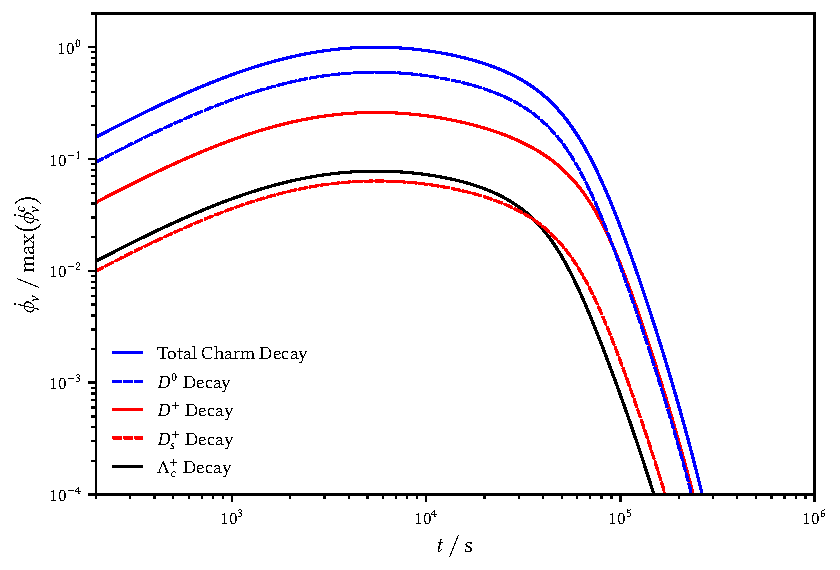
\includegraphics{../plots/build/magnetar_charm_decay_comparison_with.pdf}
	\caption[Magnetar $\nu \kern+0.5pt$ flux from $c$ decay including optical depth.]
			{Comparison of individual charmed hadron contributions to the total charm neutrino flux at
			 $E_\nu = \kern-0.5pt \qty{e9}{\giga\electronvolt}$ from a young magnetar, including the optical
			 depth defined by \eqref{eqn:optical} as a modification. Decays of $\smash{D^0}$ produce most of
			 the charmed neutrinos until later times when $\smash{D^+} \kern-0.5pt$ becomes significant, with
			 $\smash{D^+_s}$ and $\smash{\Lambda^{\kern-0.5pt +}_{\kern+0.5pt c}}$ being similar, both
			 contributing around \qty{10}{\percent} to the combined flux. This is in line with cross
			 sections and branching fractions that Sections \ref{sub:production} and \ref{sub:charm} provide.}
	\label{fig:magnetar-charm-comparison-with}
\end{figure}
